\documentclass[a4paper,11pt]{article}
\renewcommand{\baselinestretch}{1.5}
\usepackage{geometry}
 \geometry{
 a4paper,
 total={170mm,257mm},
 left=20mm,
 top=20mm,
 }

 \usepackage{wrapfig}
 \usepackage[utf8x]{inputenc}
 \usepackage{amsmath}
\usepackage{amssymb}
 \usepackage{siunitx}
 \usepackage{multirow}
\usepackage{colortbl}
 \usepackage{hhline}

 \usepackage{lipsum}  %%% Lorem ipsum

\setlength{\headheight}{30.0pt}
\setlength{\footskip}{20pt}

%%%%%%%%%%%%%%%%TABLE
\setlength{\arrayrulewidth}{0.5mm}
\setlength{\tabcolsep}{18pt}
\renewcommand{\arraystretch}{1.5}
%%%%%%%%%%%%

\usepackage{hyperref}
\hypersetup{
    colorlinks=True,
    linkcolor={blue!20!black},
    filecolor=magenta,      
    urlcolor=cyan,
}



 \usepackage[export]{adjustbox}
\usepackage[english]{babel}
\usepackage{fancyhdr}
\usepackage{multicol}

\pagestyle{fancy}
\fancyhf{}
\rhead{\textit{Pul074BEX004}}
\lhead{\textit{Amrit Prasad Phuyal}}
\rfoot{\thepage}


\usepackage{mathpazo} % Palatino font
\usepackage{graphicx}
\usepackage{float}
\usepackage{xcolor}
\usepackage{color}

%%%% Anser environment use %%%% Anser environment use %%%% Anser environment use \input{./AnsENV.tex}
%% use \begin{A... {**** argument***}
\RequirePackage{scrextend}

\newenvironment{A}[1]{\textit{Answer:}{\begin{addmargin}[2em]{2em}{#1}\end{addmargin} 
  }}

% just leave some space   
%% use \begin{A... {**** argument***}
\RequirePackage{scrextend}

\newenvironment{A}[1]{\textit{Answer:}{\begin{addmargin}[2em]{2em}{#1}\end{addmargin} 
  }}

% just leave some space   
%% use \begin{A... {**** argument***}
\RequirePackage{scrextend}

\newenvironment{A}[1]{\textit{Answer:}{\begin{addmargin}[2em]{2em}{#1}\end{addmargin} 
  }}

% just leave some space    %% Answer environment 

%%% Question Environment%%%  use 
%%% Question Environment%%%  use 
%%% Question Environment%%%  use \input{./QueENV.tex}   to include
%% Use \begin{Q}....\end{Q}

\newcounter{QC}
\setcounter{QC}{1}
\newenvironment{Q}[1]{
    \section{Question -\arabic{QC}} \stepcounter{QC}{\large\textbf{#1}}
}

%%% Question Environment%%%

   to include
%% Use \begin{Q}....\end{Q}

\newcounter{QC}
\setcounter{QC}{1}
\newenvironment{Q}[1]{
    \section{Question -\arabic{QC}} \stepcounter{QC}{\large\textbf{#1}}
}

%%% Question Environment%%%

   to include
%% Use \begin{Q}....\end{Q}

\newcounter{QC}
\setcounter{QC}{1}
\newenvironment{Q}[1]{
    \section{Question -\arabic{QC}} \stepcounter{QC}{\large\textbf{#1}}
}

%%% Question Environment%%%

 %% Question Environment 
%%%%%% include  Titles.%%%% use \input{./CP}%%%
%%%use """"""""    \CP{}{}{}{}   """" %%%% and 4 argument to craete Title page 
%%%%%%%%%%%%%%%%%%%%%%%%%%%%%%%%%%%%%%%%%%%%%%%%%%%%%%%%%%%%%%%%%
%%%argument number
%% 1=major header ## Course name 
%% 2=minor4 heading ## lab/assignmet no
%% 3=Title  ## Assignment or Lab title
%% 4=submitted to::## input receiver Name"
%%%%%%%%%%%%%%%%%%%%%%%%%%%%%%%%%%%%%%%%%%%%%%%%%%%%%%%%%%%%%%%%%


\usepackage{mathpazo} % Palatino font
\usepackage{graphicx}
\usepackage{float}

%%% format and command for lab ans c and assembly

\newcommand{\HRule}{\rule{\linewidth}{0.4mm}} % Defines a new command for horizontal lines, change thickness here



%----------------------------------------------------------------------------------------
%	TITLE PAGE
%----------------------------------------------------------------------------------------


\newcommand{\CP}[4]{ \begin{titlepage} % Suppresses displaying the page number on the title page and the subsequent page counts as page 1
		%%%%  univerdity logo%%
		\begin{figure}[H]
			\centering
			
\includegraphics[scale=0.13]{tulogo.jpg}
		\end{figure}
		%%% end university logo

		\center % Centre everything on the page

		%------------------------------------------------
		%	Headings
		%------------------------------------------------

		\textsc{\huge Institute of Engineering \\ Central Campus,Pulchowk}\\[1.5cm] % Main heading such as the name of your university/college

		\textsc{\Large #1}\\[0.5cm] % Major heading such as course name

		\textsc{\large #2}\\[0.5cm] % Minor heading such as assignment no./ lab no.

		%------------------------------------------------
		%	Title
		%------------------------------------------------

		\HRule\\[0.4cm]

		{\Huge\bfseries #3}\\[0.4cm] % Title of your document

		\HRule\\[1.5cm]

		%------------------------------------------------
		%	Author(s)
		%------------------------------------------------
		\vfill\vfill
		\begin{minipage}{0.4\textwidth}
			\begin{flushleft}
				\large{
				\textbf{Submitted BY:}\\
				{\normalsize AMRIT PRASAD PHUYAL}\\ % NAME
				{\normalsize Roll: PULL074BEX004}} % Roll
			\end{flushleft}
		\end{minipage}
		~
		\begin{minipage}{0.4\textwidth}
			\begin{flushright}
				\large
				\textbf{Submitted To:}\\
				{ \normalsize{#4}\\ }% recepent's  Name 
				{\normalsize Department of Electronics and Computer Engineering}
			\end{flushright}
		\end{minipage}

		%------------------------------------------------
		%	Date
		%------------------------------------------------

		\vfill\vfill\vfill % Position the date 3/4 down the remaining page

		{\large\today} % Date, change the \today to a set date if you want to be precise

		\vfill % Push the date up 1/4 of the remaining page

	\end{titlepage}
} %%% cover page
%%
%%% Formating And Command for Embedded Lab  VHDl
%% \ancode{caption}{Filename}


\usepackage{listings}
\usepackage{multicol}
\usepackage{mdframed}

\renewcommand{\lstlistlistingname}{List of MATLAB Codes}
\renewcommand{\lstlistingname}{MATLAB Code}

\setlength{\columnsep}{0.5cm}

\usepackage{xcolor}
\definecolor{codegreen}{rgb}{0,0.6,0}
\definecolor{codegray}{rgb}{0.3,0.3,0.3}
\definecolor{codepurple}{rgb}{0.58,0,0.82}
%\definecolor{backcolour}{rgb}{0.95,0.99,0.92}
\definecolor{backcolour}{rgb}{0,0,0}

\lstdefinestyle{MATLAB}{
  %backgroundcolor=\color{backcolour},  
  commentstyle=\color{codegreen},
  keywordstyle=\color{blue},
  numberstyle=\tiny\color{codegray},
  stringstyle=\color{codepurple},
  basicstyle=\ttfamily\small\color{black},
  breakatwhitespace=false,
  breaklines=true,
  captionpos=b,
  keepspaces=true,
  language=Matlab,
  numbers=left,
  numbersep=5pt,
  showspaces=false,
  frame = single,
  showstringspaces=false,
  showtabs=false,
  tabsize=3
}




\newcommand {\anscode}[2]{
  \lstinputlisting[style=MATLAB,nolol]{#2}

  \begingroup
  \captionof{lstlisting}{#1}
  \endgroup

}

%%% Formating And Command for Embedded Lab  VHDL %%% Matlab code
\usepackage{tikz}
\usepackage{circuitikz}
\newcommand\ddfrac[2]{\frac{\displaystyle #1}{\displaystyle #2}} 


\def\raa {R_{A}}
\def\rbb {R_{B}}
\def\vaa {V_A}
\def\vbb {V_B}
\def\va{V_1}
\def\vb{V_2}
\def\ra {R_1}
\def\rb {R_2}
\def\rc {R_3}
\def\rd {R_4}
\def\re {R_5}
\def\rf {R_6}
\def\ca {C_1}
\def\cb {C_2}

\def\Res #1{
    \SI{#1}{\ohm}
}

\newcommand{\figquestion}{
    \begin{circuitikz}
        \draw
        (0,0) to[R,l= \footnotesize$R_1\text{ = }1\text{ }\Omega$] (2,0) to [L,l=\footnotesize$L_1\text{ = }0.7654\text{ H}$] (4,0) to [C, *-*, l_=\footnotesize$C_1\text{ = }1.848 \text{ F}$] (4,-4)
        (4,0) to [L,l=\footnotesize$L_2\text{ = }1.848\text{ H}$] (8,0) to [C, *-*, l_=\footnotesize$C_2\text{ = }0.7654 \text{ F}$] (8,-4)
        (8,0) to [short] (12,0)
        (0,0) to [esource,v_=\footnotesize$V_1$] (0,-4)
        (0,-4) to [short] (12,-4) to[R, l=\footnotesize$R_2\text{ = }1\Omega$, v<=\footnotesize$V_2$] (12,0)
        ;
    \end{circuitikz}
}


\newcommand{\figfdnr}{
    \begin{circuitikz}
        \draw
        (0,0) to[C,l= \footnotesize$Z'_{R\textsubscript{$1$}}\text{ = }1\text{ F}$] (2,0) to [R,l=\footnotesize$Z'_{L\textsubscript{$1$}}\text{ = }0.7654\text{ }\Omega$] (4,0)  to [R,l=\footnotesize$Z'_{L\textsubscript{$2$}}\text{ = }1.848\text{ }\Omega$] (8,0) to [short] (12,0)
        (0,0) to [esource,v_=\footnotesize$V_1$] (0,-4)
        (0,-4) to [short] (12,-4) to[C, l=\footnotesize$Z'_{R\textsubscript{$2$}}\text{ = }1\text{ F}$, v<=\footnotesize$V_2$] (12,0)
        (4,0) to [short,*-] (4,-1.6)
        (4,-2.2) to [short,-*] (4,-4)
        (3.7,-2) node [left] {\footnotesize$Z'_{C\textsubscript{$1$}}\text{ = }1.848$}
        (8,0) to [short,*-] (8,-1.6)
        (8,-2.2) to [short,-*] (8,-4)
        (7.7,-2) node [left] {\footnotesize$Z'_{C\textsubscript{$2$}}\text{ = }0.7654$}
        ;
        \draw [thick] (3.7,-1.6)-- (4.3,-1.6);
        \draw [thick] (3.7,-1.8)-- (4.3,-1.8);
        \draw [thick] (3.7,-2)-- (4.3,-2);
        \draw [thick] (3.7,-2.2)-- (4.3,-2.2);

        \draw [thick] (7.7,-1.6)-- (8.3,-1.6);
        \draw [thick] (7.7,-1.8)-- (8.3,-1.8);
        \draw [thick] (7.7,-2)-- (8.3,-2);
        \draw [thick] (7.7,-2.2)-- (8.3,-2.2);

    \end{circuitikz}
}


\newcommand{\fighp}{
    \begin{circuitikz}
        \draw
        (0,0) to[R,l= \footnotesize$Z'_{R\textsubscript{$1$}}\text{ = }1\text{ }\Omega$] (2,0) to [C,l=\footnotesize$Z'_{L\textsubscript{$1$}}\text{ = }1.3065\text{ F}$] (4,0) to [L,l_=\footnotesize$Z'_{C\textsubscript{$1$}}\text{ = }0.5411\text{ H}$, *-*] (4,-4) (4,0) to [C,l=\footnotesize$Z'_{L\textsubscript{$2$}}\text{ = }0.5411\text{ F}$] (8,0) to [L,l_=\footnotesize$Z'_{C\textsubscript{$2$}}\text{ = }1.3065\text{ H}$, *-*] (8,-4)
        (8,0) to [short] (12,0)
        (0,0) to [esource,v_=\footnotesize$V_1$] (0,-4)
        (0,-4) to [short] (12,-4) to[R, l=\footnotesize$Z'_{R\textsubscript{$2$}}\text{ = }1\text{ }\Omega$, v<=\footnotesize$V_2$] (12,0)
        ;
    \end{circuitikz}
}


\newcommand{\figleap}{
    \begin{circuitikz}
        \draw
        (0,0) to[generic,l= \footnotesize$Z_1$,i_=\footnotesize$I_1$] (4,0) to [generic, *-*, l_=\footnotesize$Z_2$] (4,-4)
        (4,0) node (v3) [anchor=south] {\footnotesize$V_3$} to [generic,l=\footnotesize$Z_3$,i_=\footnotesize$I_2$] (8,0) (8,-4) to [generic, l=\footnotesize$Z_4$,*-*] (8,0) node (v4) [anchor=south] {\footnotesize$V_4$} to [short,-o] (9,0)
        (8,-4) to [short,-o] (9,-4)
        (0,0) to [esource,v_=\footnotesize$V_1$] (0,-4)
        (9,0) to [open,v^=\footnotesize$V_2$] (9,-4)
        (0,-4) to [short] (8,-4)
        ;
    \end{circuitikz}
}




%%%%%%%%%%%%%%%%%%%%%% for Proteus circuit  observation   supply Figure scale(1) for observation, number(2) like "a,b,c,d..", gain (3), half power freq (4),
\newcommand{\Porcirobs}[4]{
    %\subsubsection{Proteus Observation Figure #2}
    \begin{figure}[H] %%%%%%%%%%%proteus circuit
        \centering
        \includegraphics[width=\linewidth]{./FIG/P_cir_fig#2.PDF}
        \caption{Proteus Circuit for #2}
    \end{figure}


    \begin{figure}[H]  %%%%%%%%%proteus plot and observation
        \centering
        \includegraphics[width=#1\linewidth]{./FIG/plot_Fig#2.pdf}
        \begin{tabular}[H]{| m{14em}| m{22em}|}
            \hline
            \rowcolor[rgb]{0.569,0.647,0.947} \textbf{Gain } & \textbf{Half power frequency} \\ \hline
            #3 dB         & (#4) KHz     \\  \hline
        \end{tabular}
        \caption{Proteus Observation for #2}
    \end{figure}
}



\begin{document}


%%%%  COver page 
\CP{Filter Design}{Lab \#5}{DESIGN OF HIGHER ORDER ACTIVE \vfill FILTER USING
    SALLEN \& KEY BIQUAD CIRCUIT }
{SHARAD KUMAR GHIMIRE}
%%%%%%%%%%%%%%%%%%%%

\pagenumbering{gobble}
\renewcommand{\contentsname}{Table of Contents}
\tableofcontents
\vspace{5em}
%\pagebreak
\listoffigures
% \pagebreak
\vspace{5em}
\listoftables

%\lstlistoflistings

\pagebreak
\pagenumbering{arabic}

%%%%%%%%%%%%%%%%%%%%%%%%%%%%%%%%%%%%%%%%%%%%%%
\section{Title} {\large DESIGN OF HIGHER ORDER ACTIVE   FILTER USING
  SALLEN \& KEY  BIQUAD CIRCUIT}


% Objectives
\section{Objective}
\begin{itemize}
    \item To be familiar with the design of higher order active filters using cascaded biquads
    \item  To be familiar with design of filter using Sallen and Key biquad circuit
    \item  To be familiar with RC-CR transformation
\end{itemize}

%Requirement
\section{Requirement}

\subsection{Proteus Design Suite}

Proteus is a simulation and design software tool developed by Labcenter Electronics for Electrical
and Electronic circuit design.It is used to create schematic  of a circuit and
Visualization of its operation.

\pagebreak

%%Exercises

\section{Exercises:}


%Question 1
\begin{Q}
    {
        What are the different techniques to design higher order active filters? Explain.
    }
\end{Q}

Simply utilizing the first and the second order filters, higher-order filters like 3rd, 4th, 5th and so on can be made. Some popular method to realize higher order filters are:

\begin{itemize}
    \item Cascading Biquad filters
    \item Multiple-loop feedback circuit.
    \item Simulation of passive LC ladder network.
\end{itemize}

\subsubsection{Cascading Biquad filters}
In this method of Design higher order filters, the cascaded Biquad circuit along with bilinear circuit is used. Here, the requires Transfer function $Ts$ is divided into Transfer functions for Biquad and Bilinear circuit.

\begin{align*}
    T(s) = \frac{a_{m}s^m + a_{m-1}s^{m-1} + \ldots + a_0 }
    {s^n + b_{n-1}s^{n-1} + \ldots + b_0 }
\end{align*}
When $n$ is even,
\begin{align*}
    T(s) & = \prod_{i=1}^{n/2} \frac{ a_{2i}s^2 + a_{1i}s + a_{0i}}
    { s^2 + b_{1i}s + b_{0i}}       = \prod_{i=1}^{n/2}T_i(s)       \\
\end{align*}
When $n$ is odd,
\begin{align*}
    T(s) & = \ddfrac{a_{11}s+a_{01}}{s+b_{01}}
    \prod_{i=2}^{( n-1 )/2} \frac{ a_{2i}s^2 + a_{1i}s + a_{0i}}
    { s^2 + b_{1i}s + b_{0i}}  = T_1(s)\prod_{i=2}^{( n-1 )/2}T_i(s) \\
\end{align*}

The overall design of filter can be improved by allocating varying gain to the different sections of the filter. Another advantage of Cascading is Pole-zero paring where ripple is minimum in the system thus allowing factoring of Transfer function.

\begin{figure}[H]
    \centering
    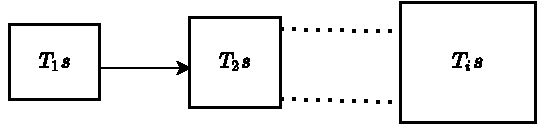
\includegraphics[width=\linewidth]{./FIG/cascade.pdf}
    \caption{Higher order filter using Cascading Biquad circuit}
\end{figure}

\pagebreak
%Question 2
\begin{Q}
    {
        From the circuit given in figure 1 derive the transfer function $ V_2(s)/V_1(s)$.
    }
\end{Q}

\begin{figure}[H]
    \centering
    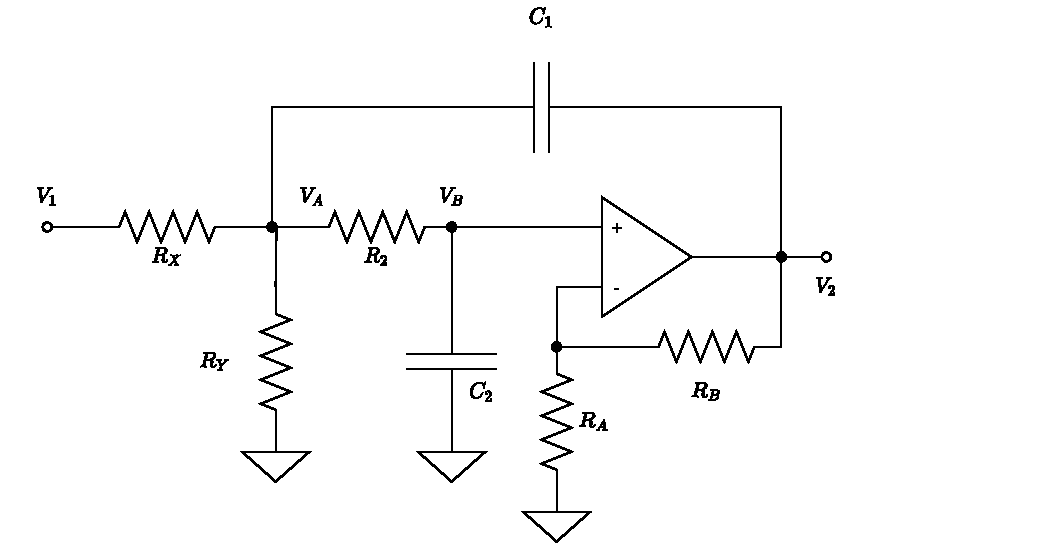
\includegraphics[width=\linewidth]{./FIG/sallenkey.pdf}
    \caption{Sallen-Key Low pass filter}
\end{figure}


For an ideal op amp, we know,
\begin{align*}
    \vbb                         & = \left( \frac{\raa}{\raa + \rbb}  \right) \vb \\
    \Rightarrow \vb              & = \left( 1 + \frac{\rbb}{\raa} \right) \vbb    \\
    \Rightarrow \vb              & = K\vbb                                        \\
    \Rightarrow  \vbb            & = \frac{\vb}{K} \numberthis                    \\
    \therefore\ddfrac{\vb}{\vaa} & =1+\ddfrac{\raa}{\rbb}=K \numberthis
\end{align*}

\begin{align*}
    \vbb             & = \frac{ 1/\cb s }{ \rb + 1/\cb s} \vaa \\
    \Rightarrow \vbb & = \frac{1}{1 + \cb s\rb} \vaa           \\\\
    \therefore \vaa  & = \frac{1+\cb s\rb}{k} \vb \numberthis
\end{align*}
Applying Nodal Analysis at $\vaa$,
\begin{align*}
    \ddfrac{\va}{\ra} + \vb(\ca s) + \frac{\vbb}{\rb} =
    \vaa \left( \frac{1}{\ra} + \frac{1}{\rb} + \ca s \right)
\end{align*}
Substituting value of $\vaa$ and $\vbb$ from above equations, we get,
\begin{align*}
    \frac{\va}{\ra} + \vb(\ca s) + \frac{\vb}{k\rb} & =
    \frac{\vb}{k} \left( \frac{(1+\cb s\rb)(\ra + \rb + \ca s\ra\rb)}{\ra\rb} \right) \\\\
    \text{or,  }
    \frac{\va}{\ra}                                 & =
    \frac{\vb}{k\ra\rb}
    \left(
    \frac{(1+\cb s\rb)(\ra + \rb + \ca s\ra\rb)} {\ra\rb}
    - sK\ra\rb\ca - \ra \right)                                                       \\\\
    \text{or,  }
    \frac{\va}{\ra}                                 & =
    \frac{\vb\ca\cb\rb}{K}
    \left( s^2 + s( \frac{1}{\rb\cb} + \frac{1}{\rb\ca}+ \frac{1}{\ra\ca}-
    \frac{k}{\rb\cb} ) + \frac{1}{\ra\rb\ca\cb} \right)                               \\
\end{align*}
Thus transfer function $ V_2(s)/V_1(s)$ is
\begin{align*}
    \label{eq:salen-final}
    \frac{\vb}{\va} =
    \cfrac{ \ddfrac {K} {\ra\rb\ca\cb }}
    { s^2 + s\left( \cfrac{1}{\rb\cb} + \cfrac{1}{\rb\ca}+ \cfrac{1}{\ra\ca}-
        \cfrac{k}{\rb\cb} \right) + \cfrac{1}{\ra\rb\ca\cb} } \numberthis
\end{align*}



\pagebreak
%Question 3
\begin{Q}
    {
        Realize the fourth order Butterworth filter (refer table 1) using Sallen-Key circuit. Perform gain
        compensation if necessary.
    }
\end{Q}

\begin{table}[H]
    \centering
    \begin{tabular}[H]{| m{8em}|m{8em}| m{8em}|m{8em}|}
        \hline
        \rowcolor[rgb]{0.569,0.647,0.947} \textbf{n=2} & \textbf{n=3}                      & \textbf{n=4}                          & \textbf{n=5}                   \\ \hline
        -0.7071068 $ \pm $ j 0.7071068                 & -0.50          $ \pm $ j 0.86603
                                                       & -0.3826834     $ \pm $ j0.9238795 & -0.809017        $ \pm $ j 0.5877852                                   \\  \hline
                                                       & -1.0                              & -0.9238795        $ \pm $ j 0.3826834 & -0.309017  $ \pm $ j 0.9510565 \\  \hline

                                                       &                                   &                                       & -1.0                           \\  \hline
    \end{tabular}
    \caption{Pole location for Butterworth Response}
\end{table}



From the table above, we can see that the pole locations for the fourth order Butterworth filter are $-0.3826834\pm j0.9238795$ and $-0.9238795\pm j0.3826834$.It has characteristic polynomial as
\begin{align*}
    H(s) = (s^2 + \num{ 0.7653 }s + 1)(s^2+\num{ 1.8478 }s + 1)
\end{align*}


The Transfer function  $ T(s)$ is cascaded form of two biquad circuit as
\begin{align}
    T(s) = T_1(s) T_2(s)=\frac{1}{ (s^2 + \num{ 0.7653 }s + 1)(s^2+\num{ 1.8478 }s + 1) }
\end{align}

where,
\begin{align}
    T_1(s) & = \frac{1}{s^2 + \num{ 0.7653 }s + 1} \label{eq:t1} \\
    T_2(s) & = \frac{1}{s^2 + \num{ 1.8478 }s + 1} \label{eq:t2}
\end{align}

We have to realise the transfer function of each circuit individually.

We have denominator for  $2^{nd}$ butterworth filter as
\begin{equation}
    s^2+s\left(\frac{\omega_o}{Q}\right)+\omega_o^2
\end{equation}
And for $T_1(s)$ when compared to equation 6, we get

\begin{align*}
    {\omega_o}         & = 1                             \\
    \frac{\omega_o}{Q} & = 0.7653 \Rightarrow Q = 1.3067 \\
    K                  & = 1
\end{align*}


For Sallen-key circuit with elemental values $C_1=C_2=1\text{ F}$ and $R_1=R_2=R$ we get,
\begin{align*}
    R = \frac{1}{\omega_o} = \Res{1} \\
    K = 3 - \frac{1}{Q} \Rightarrow K = 2.2347
\end{align*}
Form gain relation
\begin{align*}
    K                 & = 1 + \frac{\rbb}{\raa} \\
    \frac{\rbb}{\raa} & = K - 1 = 1.2347
\end{align*}

For $ \raa = \Res{1}$ and $ \rbb = \Res{1.2347}$ we need to perform gain reduction {compensation} to make gain unity. For this purpose we need Sallen-key gain reduction circuit.

\begin{figure}[H]
    \centering
    \scalebox{1.65}
    \gainred
    \caption{Gain reduction circuit for Sallen- Key}
\end{figure}


For desired gain 1,
\begin{equation}
    \begin{aligned}[b]
         & \frac{R_y}{R_x+R_y}=\frac{H}{K}=\frac{1}{2.2347}=0.4474 \\
         & \Rightarrow R_y=0.8096 R_x
    \end{aligned}
\end{equation}

From above figure,
\begin{equation}
    \begin{aligned}[b]
         & R_1=R_x||R_y=\frac{R_xR_y}{R_x+R_y} \\
         & \Rightarrow R_xR_y=R_x+R_y
    \end{aligned}
\end{equation}

Solving equation 9 an 10 we get, $R_x=2.2351\text{ }\Omega$ and $R_y=1.8095\text{ }\Omega$

Similarly for $T_2(s)$ when denominator of equation 7 compared to equation 8 we get,
\begin{align*}
    \omega_o           & = \SI{1}{\radian \per \second}  \\
    \frac{\omega_o}{Q} & = 1.8478 \Rightarrow Q = 0.5412 \\
    K                  & = 1
\end{align*}

For Sallen-key circuit with elemental values $C_1'=C_2'=1\text{ F}$ and $R_1'=R_2'=R'$we get,

\begin{equation*}
    \begin{aligned}
         & R'=\frac{1}{\omega_o'}=1 \Omega        \\
         & K'=3-\frac{1}{Q'}\Rightarrow K'=1.1522
    \end{aligned}
\end{equation*}

From gain relation,
\begin{equation*}
    \begin{aligned}
         & K'=1+\frac{R_b'}{R_a'}\Rightarrow \frac{R_b'}{R_a'}=K'-1=0.1522
    \end{aligned}
\end{equation*}


We again have to perform gain reduction to make gain unity. For this purpose we need Sallen-key gain reduction circuit as above.

For desired gain 1,
\begin{equation}
    \begin{aligned}[b]
         & \frac{R_y'}{R_x'+R_y'}=\frac{H}{K}=\frac{1}{1.1522}=0.8679 \\
         & \Rightarrow R_y'= 6.57 R_x'
    \end{aligned}
\end{equation}

From above figure,
\begin{equation}
    \begin{aligned}[b]
         & R_1'=R_x'||R_y'=\frac{R_x'R_y'}{R_x'+R_y'} \\
         & \Rightarrow R_x'R_y'=R_x'+R_y'
    \end{aligned}
\end{equation}


Solving equation 9 an 10 we get, $R_x'=1.1522 \text{ } \Omega$ and $R_y'=7.57\text{ }\Omega$


Hence final cascaded filter is shown below.
\begin{figure}[H]
    \centering
    \scalebox{1.15}
    \figfourthorder
    \caption{Fourth order butterworth lowpass filter using Sallen-Key circuit}
\end{figure}


\pagebreak
%Question 4
\begin{Q}
    {
        Obtain the final design of lowpass filter having half power frequency of 3.1831 KHz and
        practically realizable elements. Realize it in circuit and observe the magnitude response. Also note
        down the gain in passband and half power frequency.
    }
\end{Q}



For required half power frequency of 3.1831 KHz, Frequency Scaling factor $K_f$ is given by,
\begin{equation}
    K_f=\frac{\Omega}{\omega_o}=\frac{2\pi\times3.1831\times10^3}{1}\approx 20\times10^3
\end{equation}
Furthermore, Impedance scaling $K_m= 1 *10^3$ is also applied to obtain the practically realizable values.

\begin{table}[H]
    \centering
    \begin{tabular}[H]{| m{8em}|m{8em}|m{8em}|m{8em}|}
        \hline
        \rowcolor[rgb]{0.569,0.647,0.947}
        \textbf{Normalized value $1^{st}$ part}
                          & \textbf{Final Value $1^{st}$ part}
                          & \textbf{Normalized value $2^{nd}$ part}
                          & \textbf{Final Value $2^{nd}$ part}                                                     \\
        \hline
        1 $ \Omega $      & $R_a$ = 1  $ K\Omega $                  & 1 $ \Omega $      & $R_a'$=  1 $ k\Omega $   \\ \hline
        1.2347 $ \Omega $ & $R_b$ = 1.2347 $ K\Omega $              & 0.1522 $ \Omega $ & $R_b'$= 152.2 $ \Omega $ \\ \hline
        2.2351 $ \Omega $ & $R_x$ = 1  $ K\Omega $                  & 1.1522 $ \Omega $ & $R_x'$= 1  $ K\Omega $   \\ \hline
        1.8095 $ \Omega $ & $R_y$ = 1  $ K\Omega $                  & 7.57 $ \Omega $   & $R_y'$= 1  $ K\Omega $   \\ \hline
        1 $ \Omega $      & $R_2$ = 1$ K\Omega $                    & 1 $ \Omega $      & $R_2'$= 1 $ K\Omega $    \\ \hline
        1 nF              & $C_1$ = 50 nF                           & 1 nF              & $C_1'$=   50 nF          \\ \hline
        1 nF              & $C_2$ = 50 nF                           & 1 nF              & $C_2'$=    50 nF         \\ \hline
    \end{tabular}
    \caption{Component values at half power frequency $k_f =3.18 Khz$}
\end{table}

\begin{figure}[H]
    \centering
    \scalebox{1.15}
    \figfourthorderfinal
    \caption{Fourth order butterworth lowpass filter with half power frequency 3.1831 KHz}
\end{figure}


\Porcirobs{0.95}{fourth order low pass}{0}{3.177}


\pagebreak
%Question 5
\begin{Q}
    {
        Apply RC-CR transformation in your filter circuit obtained in problem C, to obtain the highpass
        filter.
    }
\end{Q}

To convert low pass filter to high pass filter, we need to apply RC-CR transformation. Here each resistor with value $R$ is replaced by a capacitor with value $\ddfrac{1}{R}$ and each capacitor with value $C$ is replaced by a resistor with value $\ddfrac{1}{C}$. Additionally we have to perform gain reduction(compensation).

\textbf{First Part}

\begin{equation}
    \begin{aligned}[b]
         & Z_x||Z_y = \frac{1}{s\times1}                                                                                          \\
         & \Rightarrow \frac{1}{s}=\ddfrac{\left(\frac{1}{sC_x}\right)\left(\frac{1}{sC_y}\right)}{\frac{1}{sC_x}+\frac{1}{sC_y}} \\
         & \therefore C_x+C_y=1
    \end{aligned}
\end{equation}

From gain relation,
\begin{equation}
    \begin{aligned}[b]
         & \frac{Z_y}{Z_x+Z_y}=\frac{1}{2.2347}=0.4474      \\
         & \Rightarrow 0.5526Z_y=0.4474Z_x                  \\
         & \Rightarrow Z_y=0.8096 Z_x                       \\
         & \Rightarrow \frac{1}{sC_y}=0.8096 \frac{1}{sC_x} \\
         & \therefore C_x=0.8096 C_y
    \end{aligned}
\end{equation}

Solving equation 14 and 15 we get, $C_x=0.4474\text{ F}$ and $C_y=0.5526\text{ F}$.

\textbf{Second Part}

\begin{equation}
    \begin{aligned}[b]
         & \frac{1}{s\times1}=Z_x'||Z_y' \\
         & \therefore C_x'+C_y'=1
    \end{aligned}
\end{equation}


From gain relation,
\begin{equation}
    \begin{aligned}[b]
         & \frac{Z_y'}{Z_x'+Z_y'}=\frac{1}{1.1522}=0.8679   \\
         & \Rightarrow 0.1321Z_y'=0.8679Z_x'                \\
         & \Rightarrow \frac{1}{sC_y'}=6.57 \frac{1}{sC_x'} \\
         & \therefore C_x'=6.57 C_y'
    \end{aligned}
\end{equation}
Solving Equation 16 and 17, we get, $C_x'=0.8679\text{ F}$ and $C_y=0.1321\text{ F}$.

Hence the high pass filter transformed using RC-CR method is shown below.

\begin{figure}[H]
    \centering
    \figfourthorderhp
    \caption{Fourth order butterworth highpass filter using RC-CR transformation}
\end{figure}

\pagebreak

%Question 6
\begin{Q}
    {
        Finally obtain a highpass filter (from the circuit obtained in problem E) having half power
        frequency of 4.775 kHz with practically realizable elements. Realize the network and observe the
        response and note down the gain in passband and half power frequency.
    }
\end{Q}


For required half power frequency $k_f =4.775 Khz$, Frequency Scaling factor $K_f$ is given by,
\begin{equation}
    K_f=\frac{\Omega}{\omega_o}=\frac{2\pi\times4.775\times10^3}{1}\approx 30\times10^3
\end{equation}
Furthermore, Impedance scaling $K_m= 1 *10^3$ is also applied to obtain the practically realizable values.

\begin{table}[H]
    \centering
    \begin{tabular}[H]{| m{8em}|m{8em}|m{8em}|m{8em}|}
        \hline
        \rowcolor[rgb]{0.569,0.647,0.947}
        \textbf{ Normalized value $1^{st}$ part}
                          & \textbf{Final Value $1^{st}$ part}
                          & \textbf{Normalized value $2^{nd}$ part}
                          & \textbf{Final Value $2^{nd}$ part}                                                     \\ \hline
        1 $ \Omega $      & $R_a$ = 1  $ K\Omega $                  & 1 $ \Omega $      & $R_a'$=  1 $ k\Omega $   \\ \hline
        1.2347 $ \Omega $ & $R_b$ = 1.2347 $ K\Omega $              & 0.1522 $ \Omega $ & $R_b'$= 152.2 $ \Omega $ \\ \hline
        1 $ \Omega $      & $R_1$ = 1  $ K\Omega $                  & 1 $ \Omega $      & $R_1'$= 1  $ K\Omega $   \\ \hline
        1 $ \Omega $      & $R_2$ = 1$ K\Omega $                    & 1 $ \Omega $      & $R_2'$= 1 $ K\Omega $    \\ \hline
        0.4474 nF         & $C_x$ = 14.913 nF                       & 0.8679 nF         & $C_x'$=   28.93 nF       \\ \hline
        0.5526 nF         & $C_y$ = 18.42 nF                        & 0.1321 nF         & $C_y'$=   4.4 nF         \\ \hline
        1 nF              & $C_2$ = 33.33 nF                        & 1 nF              & $C_2'$=    33.33 nF      \\ \hline
    \end{tabular}
    \caption{Component values at half power frequency $k_f =4.775 Khz$}
\end{table}


\begin{figure}[H]
    \centering
    \scalebox{1.15}
    \figfourthorderhpfinal
    \caption{Fourth order butterworth Highpass filter with half power frequency 4.775 KHz}
\end{figure}


\Porcirobs{0.95}{fourth order high pass}{0}{4.86}



%section for discussion and conclustion
\section{Discussion and Conclusion}
In this lab we have derived the Transfer function of Sallen-Key circuits and used it further to design a Fourth order cascaded filter using two second order biquad circuit.
We also designed a low pass filter using Sallen-Key method and use RC-CR transformation to obtain high pass of required Half power frequency hence fulfilling our Lab objective.



\end{document}